\chapter{Semantica della Logica Proposizionale Classica}
\section{Fondamenti della Semantica}
Per dare una definizione di semantica si utilizzano due princìpi guida: il 
\textbf{principio di bivalenza} e il \textbf{principio di verofunzionalità}. 

\begin{pri}[Bivalenza]
Un enunciato, in ogni circostanza, è o vero o falso.
\end{pri}

Il principio di bivalenza ha come conseguenza il principio del terzo escluso. 

\begin{pri}[Verofunzionalità, composizionalità o estensibilità]
Il valore di verità di un enunciato composto dipende solo dal valore di verità 
degli enunciati che lo compongono e dal significato del connettivo che li unisce. 
\end{pri}

Dato il principio di verosimiglianza, per dare la semantica ad un connettivo come $\land$
si deve dire qual è, sotto ogni circostanza, il valore di verità di $A \land B$, 
il quale può essere \texttt{vero} o \texttt{falso} e può dipendere solo dal valore 
di verità di $A$ e $B$ e dal significato fissato per $\land$. 
\`E necessario, ora, definire informalmente cosa sia una \textit{circostanza}: 
una \textbf{circostanza} è un assegnamento che definisce lo stato vero 
o falso di una lettera proposizionale (o di una formula), definita come 
una funzione $\mathfrak{v}$:
$$
\mathfrak{v} : L \rightarrow \{0,1\}
$$

Quindi $\mathfrak{v}(A \land B) \in \{0,1\}$ e, grazie al principio di Verofunzionalità, 
dipende solo da $\mathfrak{v}(A)$, 
$\mathfrak{v}(B)$ e dal significato fissato per $\land$, definito come 
$$
I_{\land}: \{0,1\}^2 : \{0,1\}
$$
E si ha, quindi
$$
\mathfrak{v}(A \land B ) = I_{\land} (\mathfrak{v}(A), \mathfrak{v}(B))
$$
\paragraph{Importanza della Verofunzionalità}
Si supponga per un attimo che invece di Logica si stia studiando Probabilità, 
tentando di formalizzarla come stiamo formalizzando ora la Logica Proposizionale. 
Siamo in una circostanza in cui un certo evento ha probabilità
$p(A) = \frac{1}{2}$ e un altro evento ha probabilità $p(B) = \frac{1}{2}$. 
La probabilità $p(A \rightarrow A) = 1$ rappresenta l'evento certo. 
Qual è la probabilità $p(A \rightarrow B)$? Se fossimo in una situazione verofunzionale, 
questa probabilità dovrebbe essere $1$, in quanto se $p(\frac{1}{2} \rightarrow \frac{1}{2}) = 1$, 
allora anche per $p(A \rightarrow B) = 1$. Per concretezza, si immagini 
$A = $ domani piove e $B = $ a Pasqua nevica.  In conclusione, la 
Verofunzionalità è una caratteristica stringente della Logica Proposizionale 
da non dare affatto per scontata. 

\subsection{Definizione di Semantica}
Siamo finalmente pronti per dare una definizione formale della 
\textbf{semantica} della Logica Proposizionale: 
\begin{defi}[Semantica della Logica Proposizionale]
Un assegnamento (o valutazione) è un'arbitraria funzione 
$$
\mathfrak{v} : L \rightarrow \{0,1\}
$$ 
\end{defi}
che formalizza la nozione intuitiva di circostanza (o \textit{mondo possibile}). 

\begin{defi}[Semantica dei connettivi]
        La \textbf{semantica dei connettivi} è espressa tramite delle funzioni:
$$
I_{\land} : \{0,1\}^2 : \{0,1\}
$$
\end{defi}
che identificano una \textit{tabella di verità}.

\begin{defi}[Semantica degli Enunciati]
        La \textbf{semantica degli enunciati} è l'\textbf{estensione canonica}
$$
\widetilde{\mathfrak{v}}: F_L \rightarrow \{0,1\}
$$
ossia l'estensione di $\mathfrak{v}$ a tutte le formule, definita in questo modo: 
\begin{itemize}
  \item $\widetilde{\mathfrak{v}}(p) = \mathfrak{v}(p)$ se $p \in L$
  \item $\widetilde{\mathfrak{v}}(A \land B) = I_{\land}(\widetilde{\mathfrak{v}}(A), \widetilde{\mathfrak{v}}(B))$ se $p \in F_L$
  \item $\widetilde{\mathfrak{v}}(A \lor B) = I_{\lor}(\widetilde{\mathfrak{v}}(A), \widetilde{\mathfrak{v}}(B))$se $p \in F_L$
  \item $\widetilde{\mathfrak{v}}(A \rightarrow B) = I_{\rightarrow}(\widetilde{\mathfrak{v}}(A), \widetilde{\mathfrak{v}}(B))$ se $p \in F_L$
  \item $\widetilde{\mathfrak{v}}(\neg A) = I_{\neg}(\widetilde{\mathfrak{v}}(A))$ se $p \in F_L$
\end{itemize}
\end{defi}

Vi sono inoltre delle forme algebriche per esprimere i valori di verità dei connettivi, 
per esempio 
$$
\widetilde{\mathfrak{v}}(A \rightarrow B) = min\{1-\widetilde{\mathfrak{v}}(A), \widetilde{\mathfrak{v}}(B)\}
$$
Con un poco importante abuso notazionale, si tenderà ad evitare di esplicitare 
$\widetilde{\mathfrak{v}}$ in favore della notazione $\mathfrak{v}$.
\section{Nozioni Semantiche Fondamentali}

\begin{defi}[Tautologia]
Una formula $F \in F_L$ è una tautologia se e solo se 
$$
\mathfrak{v}(F) = 1 \forall \mathfrak{v} : F_L \rightarrow \{0,1\}
$$
\end{defi}
\begin{defi}[Formula Soddisfacibile]
Una formula $F \in F_L$ è soddisfacibile se e solo se 
$$
\exists \mathfrak{v}:F_L \rightarrow \{0,1\} : \mathfrak{v}(F) = 1
$$
\end{defi}
\begin{defi}[Contraddizione]
Una formula $F \in F_L$ è una contraddizione (o insoddisfacibile, refutabile) se e solo 
se 
$$
\mathfrak{v}(F) = 0 \forall \mathfrak{v}: F_L \rightarrow \{0,1\}
$$
\end{defi}
C'è un fatto molto semplice che lega tra di loro questi concetti: 
\begin{teo}
$F \in F_L$ è una tautologia se e solo se $\neg F$ è insoddisfacibile. 
\end{teo}
\begin{proof}
  $F$ è tautologica se e solo se $\widetilde{\mathfrak{v}}(F) = 1$ per 
  ogni $\mathfrak{v}: L \in \{0,1\}$, ossia se e solo se $\widetilde{\mathfrak{v}}(\neg F) 
  = 0$ per ogni $\mathfrak{v}: L \in \{0,1\}$, ossia $\neg F$ è insoddisfacibile. 
\end{proof}

\subsection{Principio d'Induzione su $F_L$}
Benché non sia una sfaccettatura prettamente semantica, in quanto verrà 
(anzi, è già stato) utilizzato abbondantemente, è importante formalizzare 
il  \textbf{principio d'induzione}. Sia 
$P$ una proprietà delle formule; si ha che 
$P$ vale per ogni formula $F \in F_L$ se e solo se: 
\begin{enumerate}
  \item \textbf{(base):} $P$ vale per ogni $p \in L$
  \item \textbf{(passo induttivo)}: se $P$ vale per $A,B  \in F_L$, allora 
    vale anche per $\neg A$, $A \rightarrow B$, $A \lor B$ e $A \land B$. 
\end{enumerate}
Si può dimostrare induttivamente una proprietà anche grazie 
alla definizione  induttiva di $F_L$. Sia 
$$
I = \{ F \in F_L : \text{ la proprietà } P \text{ vale per } F\}
$$
vogliamo mostrare $I = F_L$, ossia che $I$ è esattamente l'insieme di tutte le formule; 
questo si dimostra mostrando che $I \subseteq F_L$ e che $F_L \subseteq I$. 
\`E ovvio, per definizione, che $I \subseteq F_L$ in quanto è definito 
come un sottoinseme di formule. Per dimostrare il contrario, si dimostra che 
$I$ soddisfa il primo punto della definizione induttiva di $F_L$, ossia contiene 
tutte le lettere proposizionali (dalla base induttiva) e anche il secondo, in  quanto 
se $A,B \in I$ allora anche $(\neg A)$, $(A \rightarrow B)$, $(A \land B)$ e 
$(A \lor B)$. Grazie al terzo punto della definizione di $F_L$, si può inoltre affermare 
che in quanto non sono contenute altre formule in $I$ (per definizione) $I = F_L$.

Come esempio, si dimostra induttivamente il seguente lemma: 
\begin{lem}[Verità di una Formula]
Sia $F \in F_L$ e siano $\mathfrak{v}, \mathfrak{v}' : L \rightarrow \{0,1\}$. 

Se $\mathfrak{v}(p) = \mathfrak{v}'(p) \forall p \in L \in F$\footnote{Per ogni letterale nell'insieme dei letterali nella formula.}, 
allora $\widetilde{\mathfrak{v}}(F) = \widetilde{\mathfrak{v}}'(F)$.
\end{lem}
\begin{proof}
  \textit{Per induzione su } $F_L$.
  \begin{itemize}
    \item \textbf{base:} Se $F = p \in L$ allora per ipotesi $\mathfrak{v}(p) = \mathfrak{v}'(p)$ e 
      anche $\widetilde{\mathfrak{v}}(p) = \widetilde{\mathfrak{v}}'(p)$.
    \item Se $F = \neg A$ allora per ipotesi induttiva 
      $\widetilde{\mathfrak{v}}(p) = \widetilde{\mathfrak{v}}'(p)$ e $\widetilde{\mathfrak{v}}(F) = 1 - 
      \widetilde{\mathfrak{v}}(A) = 1 - \widetilde{\mathfrak{v}}'(A) = \widetilde{\mathfrak{v}}'{F}$
    \item Se $F = (A \land B)$ per ipotesi induttiva $\widetilde{\mathfrak{v}}(A) = \widetilde{\mathfrak{v}}'(A)$ 
      e $\widetilde{\mathfrak{v}}(B) = \widetilde{\mathfrak{v}}'(B)$ e pertanto 
      $\widetilde{\mathfrak{v}}(F) = \min\{\widetilde{\mathfrak{v}}(A), \widetilde{\mathfrak{v}}(B)\} = 
      \min\{\widetilde{\mathfrak{v}}'(A), \widetilde{\mathfrak{v}}'(B)\} = \widetilde{\mathfrak{v}}'(F)$.
    \item uguale per gli altri connettivi.
  \end{itemize}
\end{proof}
Il lemma appena provato ci garantisce che se vogliamo calcolare $\widetilde{\mathfrak{v}}(F)$ 
ci basta calcolare la tabella di verità di $F$. A questo punto si può calcolare, 
per ogni assegnamento, se una formula è vera, soddisfacibile, tautologica o 
insoddisfacibile.

\paragraph{Esercizio}
Date $A, B \in F_L$ si esaminino le seguenti formule. 
La formula $A \land \neg A$ è insoddisfacibile, come si può osservare dalla 
sua tabella di verità nella Tabella \ref{table:insodd}.
\begin{table}[!h]
  \centering
  \begin{tabular}{|c|c|}
  \hline
  $A$ & $A \land \neg A$ \\
   0  &   0        \\ 
   1  &  0         \\
   \hline
 \end{tabular}
 \caption{}
 \label{table:insodd}
\end{table}

La formula $A \rightarrow \neg A$ è soddisfacibile ma non tautologica, 
come si può osservare dalla sua tabella di verità nella Tabella \ref{table:sodd}.
\begin{table}[h]
  \centering
  \begin{tabular}{|c|c|}
    \hline 
    $A$ & $A \rightarrow \neg A$\\
     0 &   1 \\
     1 &  0 \\
     \hline
  \end{tabular}
  \caption{}
  \label{table:sodd}
\end{table}

Si noti come è stato detto che $A,B$ siano state definite come appartenenti 
all'insieme delle formule e non alle lettere ($L$), ``imbrogliando'', un poco, 
rispetto al lemma precedente. Tuttavia, $A$ e $B$ possono essere considerate 
come \textit{metavariabili} a prescindere dalla loro complessità. Non è invece 
possibile fare il contrario, ossia considerare lettere come delle formule: 
per esempio, non è possibile dire che una lettera sia una tautologia. 

\paragraph{Esercizio}
Verificare che le seguenti siano Tautologie per ogni $A,B \in F_L$:
\begin{enumerate}
  \item $A \rightarrow (B \rightarrow A)$ (Weakening, Prefixing)
  \item $(\neg A \rightarrow A) \rightarrow A$ (Consequentia Mirabilis)
  \item $(A \rightarrow B) \lor (B \rightarrow A)$ 
  \item $(A \rightarrow B) \rightarrow (\neg B \rightarrow \neg A)$ (Contronominale)
  \item $(A \land B) \rightarrow A$
  \item $A \lor \neg A$  (Tertium non datur)
  \item $\bot \rightarrow A$ (Ex Falsum Quodlibet Sequitur)
\end{enumerate}

\begin{defi}[Tautologia]
Se la formula $F$ è una tautologia, si indicherà 
$$
\models F
$$
\end{defi}


\section{Semantica degli Insiemi di Formule}
\begin{defi}[Teoria]
Sia $\Gamma \subseteq F_L$ un insieme di formule. $\Gamma$ è detto 
\textbf{teoria} ed è un modello per un mondo in cui tutte le formule che 
gli appartengono sono vere.
\end{defi}
Si dice che $\Gamma$ è soddisfacibile 
se e solo se  
$$
\exists \mathfrak{v}: L \rightarrow \{0,1\} ~~~ \forall \gamma \in \Gamma:\mathfrak{v}(\gamma) = 1
$$
o, in notazione alternativa, $\mathfrak{v} \models \gamma$ e contestualmente 
si dice $\mathfrak{v} \models \Gamma$. Al contrario, se e solo se 
$$
\forall \mathfrak{v}: L \rightarrow \{0,1\} ~~ \exists \gamma \in \Gamma : \mathfrak{v}(\gamma) = 0
$$
la teoria $\Gamma$ è insoddisfacibile e $\mathfrak{v} \nvDash \gamma$ e 
$\mathfrak{v} \nvDash \Gamma$. 

\begin{defi}[Conseguenza Logica]
Sia $\Gamma \subseteq F_L$ e $A \in F_L$. La formula $A$ è una 
\textbf{conseguenza logica} di $\Gamma$ se e solo se 
$$
\forall \mathfrak{v}: L \rightarrow \{0,1\} : \mathfrak{v} \models\gamma \in \Gamma
$$ 
(quindi $\mathfrak{v} \models\Gamma$) e $\mathfrak{v} \models A$. 
Si denoterà questo fatto con la notazione $\Gamma \models A$.
\end{defi}

\paragraph{Esercizio} 
Esprimere il concetto di formula tautologica o tautologia ($\models A$)
attraverso il concetto di conseguenza logica. 
Quando si ammette una teoria, si restringe il campo dei possibili assegnamenti. 
Una formula è tautologica quanto è vera in ogni circostanza ed è verificata 
da ogni assegnamento. Sia $\Gamma$ definito in questo modo. $\Gamma \subseteq F_L$ 
un insieme composto solo da tautologie. Allora 
$\Gamma \models A$. Dato che è sempre meglio avere come teoria la più semplice 
possibile, si può definire $\Gamma = \emptyset$, concludendo $\emptyset \models A$. 

\noindent
Ogni tanto si può utilizzare la notazione $\Gamma \cup \{A\} \models B$, che 
a volte viene semplificato in $\Gamma,A \models B$. 

\subsection{Proprietà semantiche fondamentali delle Teorie}

\begin{lem}[Conseguenza Logica di una Formula da una Teoria insoddisfacibile]
Sia $\Gamma \subseteq F_L$ una teoria e $A \in F_L$. Si 
ha che $\Gamma \models A$ se e solo se $\Gamma \cup \{\neg A \}$ è insoddisfacibile. 
\end{lem}

\begin{proof}
Dimostriamo che $\Gamma \models A$ se e solo se 
$\mathfrak{v} \models \gamma \forall \gamma \in \Gamma \rightarrow \mathfrak{v}\models A$, 
in altre parole per ogni assegnamento di verità tale che $\mathfrak{v} \models \Gamma$ 
si ha $\mathfrak{v}(A) = 1$.
Si può tradurre quanto scritto utilizzando la definizione di implicazione materiale, 
ossia 
\begin{align*}
  &\neg (\mathfrak{v} \models \gamma \forall \gamma \in \Gamma) \lor \mathfrak{v}\models A \\
  \iff &\neg (\mathfrak{v}(\gamma) = 1 \forall \gamma \in \Gamma) \lor \mathfrak{v}(A) = 1\\
  \iff & (\exists \gamma \in \Gamma : \mathfrak{v}(\gamma) = 0) \lor \mathfrak{v}(\neg A) = 0 \\
  \iff & \exists B \in \Gamma \cup \{\neg A\}: \mathfrak{v}(B) = 0  \\
  \iff & \Gamma \cup \{\neg A\} \text{ è insodd.}
\end{align*}
\end{proof}

\begin{lem}[Deduzione, semantico] Siano $P$, $Q$ due formule. Allora 
si dice che $P \models Q$ se e solo se $\models P \rightarrow Q$. 
\end{lem}
\begin{proof}
Assumiamo che $P \models Q$. Per definizione, 
$\forall \mathfrak{v}: L \rightarrow \{0,1\}:\mathfrak{v}(P) = 1 \rightarrow \mathfrak{v}(Q) = 1$. 
Assumendo, quindi, che ogni volta che $\mathfrak{v}(P) = 1$ si ha $\mathfrak{v}(Q) = 1$, 
si ha direttamente che $\models P\rightarrow Q$, in quanto sostanzialmente 
si rimuove la possibilità di avere $P$ vero e $Q$ falso.
\end{proof}

Il teorema generalizza il lemma alla seguente situazione. 
\begin{teo}[Deduzione,semantico]
Sia $\Gamma$ una teoria 
e $P$, $Q$ formule. Allora $\Gamma,P \models Q$ se e solo se
$\Gamma \models P \rightarrow Q$. 
\end{teo}
\begin{proof}
Si dimostra dicendo che $\Gamma, P \models Q$ se e solo se 
$\forall \mathfrak{v}: L \rightarrow \{0,1\}: \mathfrak{v}(\gamma) = 1 \forall \gamma \in \Gamma$ e 
$\mathfrak{v}(P) = 1$ si ha che $\mathfrak{v}(Q) = 1$. Questo avviene se e solo se 
$\forall \mathfrak{v}:L \rightarrow \{0,1\} : \mathfrak{v}(\gamma) = 1$ si ha $\mathfrak{v}(P \rightarrow Q) = 1$ 
e segue per definizione $\Gamma, P \models Q$. 
\end{proof}

\subsection{Teorema di Compattezza}
Il teorema di compattezza è un teorema fondamentale della logica e varrà 
anche per la logica del prim'ordine. Lo proviamo ora per la logica proposizionale. 
\`E in qualche modo, in forma astratta, un teorema di completezza. 

Prima di mostrare l'enunciato, si introduce il concetto. \`E stata data la 
nozione di teoria, $\Gamma \subseteq F_L$: ci si chiede se serve, nella logica 
proposizionale, considerare teorie infinite (composte da un numero 
infinito di formule). A priori, sembrerebbe proprio di sì - d'altronde $F_L$ è di 
cardinalità numerabile - e si vedrà affrontando
la Logica dei Predicati che una singola formula al Prim'Ordine contiene informazioni 
di un numero infinito di formule proposizionali; questo basta per giustificare il caso 
in cui $\Gamma$ sia una teoria infinita. Il punto è che non sembra possibile 
gestire la teoria infinita: qui torna utile il teorema di compattezza. 
 

Il teorema di compattezza permette di ridurre l'analisi della soddisfacibilità di 
una teoria eventualmente infinita all'esame della soddisfacibilità dei suoi 
sottoinsiemi finiti. Tuttavia, è ovvio che il numero di sottoinsiemi finiti 
sia infinito. 
\noindent

Si enuncia, ora, il teorema di compattezza.
\begin{teo}[Compattezza]
Un insieme $\Gamma \subset F_L$ è soddisfacibile se e solo se lo è ogni
$\Gamma' \subseteq \Gamma$, con $\Gamma'$ finito, con notazione: $\Gamma' \subseteq_{\omega} \Gamma$ (leggasi 
``$\Gamma '$ sottoinsieme finito di $\Gamma$'').
\end{teo}
La dimostrazione consiste nel 
provare che 
che se ogni $\Gamma ' \subseteq_{\omega} \Gamma$ è 
soddisfacibile allora lo è anche $\Gamma$, in quanto l'altro 
verso è ovvio dalla definizione di soddisfacibilità di una teoria, mentre
il fatto che sottoinsiemi di $\Gamma$ siano soddisfacibili non implica ovviamente 
che $\Gamma$ sia soddisfacibile. 

\subsubsection{Dimostrazione}
Per prima cosa, si definisce una porzione di terminologia utile per la 
dimostrazione. 
\begin{defi}
        Definiamo $\Gamma$ \textit{finitamente soddisfacibile} (fin. sodd.) 
        se per ogni $\Gamma' \subseteq_{\omega} \Gamma$ 
        si ha che $\Gamma'$ è soddisfacibile.
\end{defi}

Il succo della dimostrazione sarà la relazione tra 
finitamente soddisfacibile e soddisfacibile, ossia 
si proverà che $\Gamma$ fin. sodd. implica $\Gamma$ soddisfacibile. 

Fissato una successione 
$$
F_1, F_2, \cdots, F_k, \cdots
$$ 
senza ripetizioni di tutte le formule in $F_L$ ($F_i \in F_L$), si costruisce una successione 
infinita di insiemi di formule 
$$
D_0, D_1, \cdots, D_k, \cdots
$$ 
definita induttivamente sull'indice $i$ di $D_i$. Sia 

$$
\begin{cases}
        D_0 = \Gamma \\
        D_{n+1} = 
        \begin{cases} 
          D_n \cup \{F_{n+1}\} & \text{se } D_n \cup \{F_{n+1}\} \text{ è finitamente soddisfacibile} \\
          D_n \cup \{\neg F_{n+1}\} & \text{altrimenti}
        \end{cases}
\end{cases}
$$

Bisogna sottolineare che la definizione di $D_n$ non garantisce, a priori, 
che ogni $D_n$ sia finitamente soddisfacibile, anche se si dimostrerà che è 
in effetti così. In altre parole, definire $D_n = D_{n-1} \cup \{\neg F_{n+1}\}$ 
se l'alternativa non è finitamente soddisfacibile, non ci assicura a priori che 
$D_n$ sia fin. sodd.; per arrivare a tale conclusione è necessaria una 
dimostrazione.
Si definisce infine
$$
D = \bigcup_{i \in \mathbb{N}} D_i
$$
Prima di passare alle effettive dimostrazioni, si noti come per dimostrare 
una proprietà di $\Gamma$ stiamo cercando di dimostrare qualcosa di relativo a 
un insieme infinitamente più grande, $D$; benché questa possa sembrare un'idea 
balzana, il Teorema di Compattezza ci dimostrerà che questo è il procedimento 
giusto per ottime ragioni. 

\paragraph{Primo fatto:}
Per dimostrare che $D_n$ sia fin. sodd. per ogni $n$ ci si basa sull'induzione 
sull'indice $n$. 
Per la base dell'induzione, 
$D_0 = \Gamma$ è finitamente soddisfacibile per ipotesi. Per $n \neq 0$, si suppone 
che questo fatto sia vero per $D_0, \cdots, D_n$ e si prova vero per $D_{n+1}$. 

Per mostrare $D_{n+1}$ finitamente soddisfacibile si procede per assurdo: si assume 
$D_{n+1}$ non finitamente soddisfacibile in modo di arrivare ad una contraddizione. 
Se $D_{n+1}$ non è finitamente soddisfacibile,
allora esiste un insieme $D' \subseteq_{\omega} D_{n}\cup \{F_{n+1}\}$ 
tale che $D'$ è insoddisfacibile ed esiste $D''\subseteq_{\omega} D_{n} \cup \{\neg F_{n+1}\}$
tale che $D''$ è insoddisfacibile. 

Senza perdita di generalità, si può assumere che 
$$
F_{n+1} \in D' \text{ e } \neg F_{n+1} \in D''
$$
in altre parole $D' = E' \cup \{F_{n+1}\}$ e $D'' = E'' \cup \{\neg F_{n+1}\}$. 
Si può affermare che $E', E'' \subseteq D_{n}$ e $F_{n+1} \notin E'$, $\neg F_{n+1} \notin E''$.
Per concludere la dimostrazione del 
fatto, si noti che 
$$
E' \cup E'' \cup \{F_{n+1}\} \text{ e } E' \cup E'' \cup \{\neg F_{n+1}\}
$$ 
sono insoddisfacibili perché contengono $D'$ e $D''$ rispettivamente.
Ma $E' \cup E'' \subseteq_{\omega} D_{n}$ e per ipotesi induttiva $D_n$ è 
finitamente soddisfacibile, ed è quindi $E' \cup E''$ soddisfacibile ed esiste 
un assegnamento tale che $\mathfrak{v} \models E' \cup E''$. Sappiamo che 
$\mathfrak{v}(F_{n+1})$ è uguale a $0$ o a $1$ e pertanto non è possibile che entrambi
$\{F_{n+1}\}$ e $\{\neg F_{n+1}\}$ siano falsi. 
Abbiamo raggiunto la contraddizione che conclude la prova per assurdo 
mostrando $D_{n+1}$ finitamente soddisfacibile. Questo chiude a sua volta la 
prova per induzione, mostrando che ogni $D_n$ per $n \in N$ è finitamente 
soddisfacibile. 
 
\paragraph{Secondo fatto:}
$D = \cup_{i \in \omega} D_i$ è a sua volta finitamente 
soddisfacibile. Questo non è necessariamente ovvio a partire dal fatto 
che $D$ sia l'unione di insiemi finitamente soddisfacibili.
Si consideri un sottoinsieme finito $D' \subseteq_{\omega} D$. Per dimostrare 
che $D'$ sia soddisfacibile (e, vista la generalità, ogni insieme $D'$ lo sia, 
quindi $D$ sia soddisfacibile), si può pensare di elencarne 
i membri $D' = \{F_{i_1}, F_{i_2},\cdots,F_{i_u}\}$. Sia $k = \max_{j=1,...,u} i_j$ 
l'indice massimo. Allora, $D' \subseteq_{\omega} D_k$, ma per il primo fatto $D_k$ è
finitamente soddisfacibile e si può concludere $D'$ soddisfacibile
e $D$ finitamente soddisfacibile.

\paragraph{Terzo fatto:}
Il terzo fatto da dimostrare è che per ogni formula o enunciato $F_t$ esattamente 
una tra $F_t$ e $\neg F_t$ appartiene a $D$. Anche questo non è necessariemente 
garantito, in quanto $F_{n+1}$ e $\neg F_{n+1}$ non hanno lo stesso indice, 
ossia $\neg F_{n+1}$ non ha indice ${n+1}$. La dimostrazione di questo fatto 
arriva col  ragionamento seguente: per costruzione della sequenza dei $D_i$ 
$F_t$ o $\neg F_t$ appartiene a $D_t$ e quindi, dato che ogni $D_t \subseteq D$ 
si ha $F_t \in D$ o $\neg F_t \in D$. Bisogna escludere che ci siano entrambe, 
e che quindi la congiunzione ``o'' diventi uno xor. Si ha che $\{F_t, \neg F_t\} \nsubseteq D$, 
perché altrimenti per il secondo fatto $D$ è finitamente soddisfacibile e si avrebbe 
che $\{F_t, \neg F_t\}$ è soddisfsacibile, ma è assurdo, dato che ovviamente 
non può essere soddisfacibile per la semantica della negazione. 

\paragraph{Quarto fatto:}
Infine, si definisce l'assegnamento $\mathfrak{v}_D : L \rightarrow \{0,1\}$:
per ogni $p \in L$ si ha $\mathfrak{v}_D(p) = 1 \iff p \in D$. Si noti che 
$\mathfrak{v}_D$ è ben 
definito in quanto necessarimente $p \in D$ o $p \notin D$. L'ultimo fatto 
afferma che $\mathfrak{v}_D \models D$, che significa che $\forall F \in D \mathfrak{v}_D(F) = 1$. 
Se questo fatto è vero, allora è vero che $\mathfrak{v}_D \models \Gamma$ dato che $\Gamma \subseteq D$, 
dunque $\Gamma$ è soddisfacibile.
Questo fatto si dimostra per induzione 
strutturale l'affermazione seguente: per ogni $F \in F_L$ si ha $\mathfrak{v}_D(F) = 1$ se 
e solo se $F \in D$. Questo non è uguale alla definizione precedente, in quanto 
in principio è stato definito per le lettere proposizionali e non per la 
funzione estesa ($\tilde{\mathfrak{v}}_D$). Ci basterebbe provare che $F \in D$ 
implica $\mathfrak{v}_D(F) = 1$ ma per convenienza proviamo anche che 
$\mathfrak{v}_D(F) = 1$ implica $F \in D$. 

La base induttiva è $F = p$ e $p \in L$, l'asserto da 
provare segue dalla definizione di $\mathfrak{v}_D$. Il passo induttivo si svolge esaminando 
i connettivi uno per volta. Se $F = \neg G$, allora 
$\mathfrak{v}_D(F) = 1 \iff \mathfrak{v}_D(G) = 0 \iff G \notin D \iff \neg G \in D \text{ dal fatto tre }\iff F \in D$. 

Se $F = (G \land H)$ allora $\mathfrak{v}_D(F) = 1 \iff \mathfrak{v}_D(G \land H) = 1 \iff \mathfrak{v}_D(G) = 1 \land \mathfrak{v}_D(H) = 1\iff G \in D \land G \in D$. Questo ultimo fatto è dimostrabile perché se $G, H \in D$ allora 
$G \land G \in D$, poiché altrimenti se $\neg(G \land H) \in D$ implicherebbe 
che $\{G, H, \neg \{G \land H\}\} \subseteq_{\omega} \in D$ finitamente 
soddisfacibile, assurdo; e se $G\land H \in D $ allora $G, H \in D$, poichè altrimenti 
$G \notin D$ o $H \notin D$. Questo implica che $\{G\land H, \neg G\}$ 
o $\{G\land H, \neg H\} \in D$ siano finitamente soddisfacibili, assurdo. 
 
Se $F = (G \lor H)$ allora $\mathfrak{v}_D(F) = \mathfrak{v}_D(G \lor H) \iff \mathfrak{v}_D(G) = 1 \lor \mathfrak{v}_D(H) = 1 \iff G \in D \text{ o } H \in D$
allora se $G \in D$ o $H \in D$, si ha che $(G \lor H) \in D$ poiché altrimenti 
se $(G \lor H) \notin D$ allora $\neg (G \lor H) \in D$, e se $G \in D$ allora 
$\{G, \neg \{G \lor H \}\} \subseteq_{\omega} D$
o se $H \in D$ allora $\{H, \neg \{G \lor H\}\} \subseteq_{\omega} D$ finitamente 
soddisfacibili, assurdo. 
Se $G \lor H \in D$ allora $G \in D$ o $H \in D$, 
poiché altrimenti se $G \notin D$ e $H \notin D$ allora $\neg G \in D $ e 
$\neg H \in D$ e $\{\neg G, \neg H, \{G \lor H \}\} \subseteq_{\omega} D$ 
finitamente soddisfacibile, impossibile. 

\subsubsection{Dimostrazione della contronominale}
$\Gamma$ è insoddisfacibile se 
e solo se esiste $\Gamma' \subseteq_{\omega} \Gamma$ e $\Gamma'$ è 
insoddisfacibile. 
\paragraph{$\leftarrow$ contronominale} 
Se c'è $\Gamma' \subseteq_{\omega} \Gamma$ insoddisfacibile, allora $\Gamma$ 
è insoddisfacibile in quanto $\Gamma$ è più restrittivo di $\Gamma'$, ha 
meno assegnamenti di $\Gamma'$ che possono soddisfarlo. 

\paragraph{$\rightarrow$ contronominale}
Se $\Gamma$ è insoddisfacibile, allora esiste $\Gamma' \subseteq_{\omega} \Gamma$, 
$\Gamma'$ insoddisfacibile. 

\subsection{Osservazioni sul Teorema di Completezza}
L'idea di dimostrare la validità del teorema di compattezza partendo 
da una teoria composta da un insieme infinito di formule per creare una catena 
di insiemi 
$$
\Gamma = D_0 \subseteq D_1 \subseteq D_2 \cdots \subseteq D_k \cdots \subseteq D
$$
è curioso. Si può concludere inoltre che $D$ non può essere ulteriormente ampliato 
senza perderne la soddisfacibilità, in quanto se $F \notin D$, allora $\overline{D} = D \cup \{F\}$ 
non è soddisfacibile: $F \notin D$ implica $\neg F \in D$.
Questo vuol dire che $D$ è un \textbf{ampliamento massimale} di $\Gamma$. 

\begin{defi}[Insieme massimale soddisfacibile]
  Si definisce \textbf{insieme massimale soddisfacibile} 
  ogni sottoinsieme $E \subseteq F_L$ tale che 
$E$ è soddisfacibile e $\forall F \in F_L : F\notin E$ si ha che $E \cup \{F\}$ è 
non soddisfacibile. 
\end{defi}
$D$ è solo uno di tali insiemi ed è quello che è stato 
costruito a partire da $\Gamma$. $D$ è un ampliamento massimale di $\Gamma$ o 
\textit{un} ampliamento di $\Gamma$? 
Pragmaticamente, se si elencano le formule in modo differente si ottiene, in genere, 
un ampliamento differente.
A livello delle informazioni contenute, un insieme massimale soddisfacibile $D$ 
si comporta come un assegnamento. Per ogni assegnamento $\mathfrak{v} : L \rightarrow \{0,1\}$ 
si può creare $D_\mathfrak{v} = \{ F \in F_L : \mathfrak{v}(F) = 1\}$, un 
insieme massimale soddisfacibile. 
Il teorema di compattezza verrà usato per decidere i casi in cui $\Gamma \models A$. 
Infatti, per un lemma che abbiamo già dimostrato, $\Gamma \models A \iff \Gamma \cup \{\neg A \} $
è insoddisfacibile. Si supponga che $\Gamma$ sia una teoria finita, 
$\Gamma = \{B_1, \cdots, B_n\}$ e si vuole sapere se $\Gamma \models A$. 
Questo è vero se e solo se $B_1, \cdots, B_n \models A \iff \{B_1, \cdots,B_n,\neg A\}$ è 
insoddisfacibile, se e solo se $B_1 \land \cdots B_n \land \neg A$ è 
insoddisfacibile. Se, invece, $\Gamma$ è infinito viene finalmente in 
nostro aiuto il teorema di compattezza. 

\section{Equivalenza Semantica}
Sintatticamente, come enunciati, cioè come stringhe di simboli, le 
due formule 
$$
A \lor B
$$ 
e 
$$
B \lor A 
$$ 
sono due formule differenti, nonostante $A$ sia $A$ e $B$ 
sia $B$: sono \textit{scritte} in modo diverso. Il loro \textbf{significato}, 
tuttavia, è uguale e, pertanto, per ogni $\mathfrak{v} : L \rightarrow \{0,1\}$ si ha che 
$\mathfrak{v}(A \lor B) \equiv \mathfrak{v}(B \lor A)$. Quella appena 
definita è una \textbf{relazione}. 

\begin{defi}[Relazione]
  Una relazione $n$-aria $R$ su un insieme $S$ è 
un sottoinsieme dell'insieme di tutte le $n$-ple di tutti gli elementi di $S$, 
in altre parole $R \subseteq S^{n}$.
\end{defi}
Per esempio, una relazione binaria è 
una relazione $R$ su $S$ tale che $R \subseteq S^2$. 
\begin{defi}[Relazione di equivalenza]
Una 
\textbf{relazione d'equivalenza} è una relazione binaria $R$ su $S$, $R \subseteq S^2$ 
tale che 
\begin{itemize}
  \setlength\itemsep{0pt}
  \item $R$ è riflessiva: $\forall s \in S ~~(s,s) \in R$
  \item $R$ è simmetrica: $\forall s_1, s_2 \in S ~~ (s_1, s_2) \in R \rightarrow (s_2, s_1) \in R$
  \item $R$ è transitiva: $\forall s_1, s_2, s_3 \in S ~~ (s_1, s_2), (s_2, s_3) \in R \rightarrow (s_1, s_3) \in R$
\end{itemize}
\end{defi}

\subsection{Partizioni e classi di equivalenza}
Sia $R$ una relazione di equivalenza su $S$. Per ogni $s \in S$, la 
\textbf{classe di equivalenza} rispetto ad $R$ di $s \in S$ è definita 
$$
[s]_R = \{ t \in S : (s,t) \in R\}
$$
\`E importante osservare che se $(s,t) \in R$ allora $[s]_R = [t]_R$ e viceversa, 
ossia se $[s]_R = [t]_R$ allora $(s,t) \in R$.  Una \textbf{partizione} di 
un insieme $S$ è un insieme $\{B_1, \cdots, B_k, \cdots\}$ non necessariamente 
finito di sottoinsiemi di $S$ ($B_i \subseteq S$) tale che $B_i \cap B_j = \emptyset$ 
per ogni $i,j \in I$, dove $I$ è l'insieme di indici di $B$. Inoltre, 
$\cup_{i \in I} B_i = S$. Gli insiemi $B_i$ vengono chiamati \textit{blocchi}
della partizione. I due concetti, partizioni e relazioni di equivalenza, sono 
legati tra di loro: ogni relazione di equivalenza $R$ su $S$ determina una partizione 
$P_R$ di $S$ dove 
$$
P_R = \{[s]_R : s \in S\}
$$
ossia le classi di equivalenza definite da $R$. La relazione inversa è meno nota, 
ossia che ogni partizione $P$ di $S$ determina una relazione d'equivalenza $R_P$ 
su $S$, ossia 
$$ 
R_P := (s,t) \in R_p \implies \exists i : s,t \in B_i
$$
che è chiaramente riflessiva, simmetrica e transitiva. 

\subsection{Equivalenza Logica}
Verificare che la relazione seguente (equivalenza logica $\equiv$) è d'equivalenza: 
$$ 
\equiv \subseteq F_L^2
$$
$$
\forall A,B: (A,B) \in \equiv \forall \mathfrak{v}:L\rightarrow \{0,1\} \mathfrak{v}(A) = \mathfrak{v}(B)
$$
\begin{enumerate}
  \item $\equiv$ riflessiva: $A \equiv A$ infatti $\forall \mathfrak{v}:L \rightarrow \{0,1\} \mathfrak{v}(A) = \mathfrak{v}(A)$
  \item $\equiv$ simmetrica: per ogni $(A,B) \in F_L^2$ se $A \equiv B$ allora
    $B \equiv A$, ossia se per ogni assegnamento $\mathfrak{v}:L \rightarrow \{0,1\}$ si 
    ha che $\mathfrak{v}(A) = \mathfrak{v}(B)$ allora per ogni $v$ si ha $\mathfrak{v}(B) = \mathfrak{v}(A)$. 
  \item $\equiv$ transitiva: per ogni $(A,B,C) \in F_L^3$ se $A \equiv B$ e 
    $B \equiv C$ allora $A \equiv C$ (dalla transitività della funzione 
    $=$ stessa). 
\end{enumerate}

$\equiv$ partiziona $F_L$, infatti 
$$
P_{\equiv} = F_L/\equiv =  \{ [A]_{\equiv} : A \in F_L\}
$$
\noindent 
\subsection{Sostituzione di lettera proposizionale con Formula}
Arricchiremo l'insieme delle classi di equivalenza delle formule, rispetto 
all'equivalenza logica, con delle operazioni che equipaggeranno tale insieme 
di una struttura algebrica.
Siano $A, B \in F_L$ delle formule e sia $p \in L$ una lettera proposizionale. 
Si definisce la formula che si ottiene sostituendo nella formula $A$ ogni 
occorrenza della lettera proposizionale $p$ con la formula $B$
$$
A[B/p]
$$
induttivamente, con l'idea che per esempio data $(p \land \neg q)$ si ha 
$[(t \rightarrow q)/p] = (t\rightarrow q) \land \neg q$. 
\newline
\textbf{base:} $A = q, p \in L$  allora 
\begin{align*}
  q[B/p] := 
  \begin{cases}
    B & p = q \\
    q & p \neq q 
  \end{cases}
\end{align*}
\newline
\textbf{passo:}  
$(\neg A)[B/p] := \neg(A[B/p])$, 
$(A_1 \land A_2)[B/p] := (A_1[B/p]) \land (A_2[B/p])$, 
$(A_1 \lor A_2)[B/p] := (A_1[B/p]) \lor (A_2[B/p])$, 
$(A_1 \implies A_2)[B/p] := (A_1[B/p] \implies A_2[B/p])$. 

\begin{lem}[di sostituzione]
Sia $\mathfrak{v}: L \rightarrow \{0,1\}$ e siamo $S,T \in F_L$. 
Se $\mathfrak{v}(S) = \mathfrak{v}(T)$,  allora per ogni $A \in F_L$ e ogni $p \in L$
$$
\mathfrak{v}(A[S/p]) = \mathfrak{v}(A[T/p])
$$ 
\end{lem}
ossia, se si sostituisce nella stessa formula una lettera proposizionale 
con due enunciati che hanno lo stesso valore di verità il valore delle due 
sostituzioni è uguale. La dimostrazione è per induzione strutturale su $A$: 
\newline 

\textbf{base:} $ A = q$, $q \in L$ allora 
\begin{align*}
  \begin{cases}
    q \neq p & q[S/p] = q = q[T/p] \\
    q = p & q[S/p] = S \land q [T/p] = T, \mathfrak{v}(S) = \mathfrak{v}(T) \rightarrow \mathfrak{v}(q[S/p]) = \mathfrak{v}(q[T/p])
  \end{cases}
\end{align*}
\newline 

\textbf{passo}: $A= \neg B$ per ipotesi induttiva $\mathfrak{v}(B[S/p]) = \mathfrak{v}(B[T/p])$, 
e quindi $\neg \mathfrak{v}(B[S/p]) = \neg \mathfrak{v}(B[T/p])$. Analogamente per gli 
operatori binari: 
$A = (B \land C)$ e per i.h. $\mathfrak{v}(B[S/p]) = \mathfrak{v}(B[T/p])$ e $\mathfrak{v}(C[S/p]) = \mathfrak{v}(c[T/p])$ 
e quindi $\mathfrak{v}((B\land C)[S/p]) = \mathfrak{v}(B[S/p] \land C[S/p])$. 

Grazie al lemma di sostituzione si può provare il seguente teorema. 
\begin{teo}[di sostituzione]
Se $S \equiv T$, allora per ogni $A \in F_L$ e $p \in L$ vale 
$$ 
A[S/p] \equiv A[T/p]
$$ 
\end{teo}
La differenza arriva dall'utilizzo di un solo assegnamento nel lemma e 
dall'utilizzo di equivalenza in questo teorema. 
La dimostrazione è ovvia grazie alla definizione di equivalenza e dal 
lemma di sostituzione. Ricordando che per ogni $\mathfrak{v}: L \rightarrow \{0,1\}$ vale 
$\mathfrak{v}(S) = \mathfrak{v}(T)$ in quanto per ipotesi $S \equiv T$ si ha che 
per il lemma di sostituzione vale 
$$
\forall \mathfrak{v}: L \rightarrow \{0,1\} \mathfrak{v}(A[S/p]) = \mathfrak{v}(A[T/p])
$$ 
dunque, per la definizione di $\equiv$ si ha $A[S/p] \equiv A[T/p]$. 


\noindent 
\subsection{Teoremi di equivalenze logiche}
Date $F, G, H \in F_L$ le seguenti sono equivalenze logiche: 

\noindent
\textbf{idempotenza:} 
$$
\begin{cases}
  F \lor F \equiv F \\
  F \land F \equiv F
\end{cases}
$$
\noindent 
\textbf{commutatività:}
$$
\begin{cases}
  F \lor G \equiv G \lor F \\
  F \land G \equiv F \land F 
\end{cases}
$$
\noindent 
\textbf{associatività:}
$$
\begin{cases}
  F \land (G \land H) \equiv (F \land G) \land H \\
  F \lor (G \lor H) \equiv (F \lor G) \lor H 
\end{cases}
$$
\noindent 
\textbf{assorbimento:}
$$
\begin{cases}
  F \lor (F \land G) \equiv F \\
  F \land (F\lor G) \equiv F 
\end{cases}
$$
\noindent 
\textbf{distributività:}
$$
\begin{cases}
  F \land (G \lor H) \equiv (F \land G) \lor (F \land H) \\
  F \lor (G \land H) \equiv (F \lor G) \land (F \lor H)
\end{cases}
$$
\noindent 
\textbf{doppia negazione:}
$$
\neg\neg F \equiv F 
$$
\noindent 
\textbf{leggi di De Morgan:}
$$
\begin{cases}
  \neg (F \lor G) \equiv \neg F \land \neg G \\
  \neg (F \land G) \equiv \neg F \lor \neg G 
\end{cases}
$$
\noindent 
\textbf{interdefinibilità:}
$$
\begin{cases}
  F \rightarrow G \equiv  (\neg F) \lor G \\
  F \rightarrow G \equiv \neg(F \land \neg G) \\
  F \lor G \equiv (\neg F) \rightarrow G \\
  F \land G \equiv \neg(F \rightarrow G) \\
  F \lor G \equiv \neg (\neg F \land \neg G) \\
  F \land G \equiv \neg(\neg F \lor \neg G)
\end{cases}
$$
\noindent 
\textbf{doppia implicazione}
$$
F \iff G \equiv (F \rightarrow G) \land (G \rightarrow F)
$$
\noindent
\textbf{tautologia iff.}
$$
\models F \iff G \iff F \equiv G
$$
\noindent 
\textbf{costanti logiche}
$$
\begin{cases}
  \bot :=  I_{\bot} : \{0,1\}^0 \rightarrow \{0,1\} \text{ la funzione costante } I_{\bot} =  0 \\
  \top :=  I_{\top} : \{0,1\}^0 \rightarrow \{0,1\} \text{ la funzione costante } I_{\top} =  1 \\
\end{cases}
$$
come primitivi oppure, come derivati
$$
\begin{cases}
  \bot := (\neg \top) \text{ oppure } p \land \neg p \\
  \top := (\neg \bot) \text{ oppure } p \rightarrow p, p \lor \neg p \\
  \neg A \equiv A \implies \bot \\
  A \equiv \top \implies A 
\end{cases}
$$
\noindent 
\textbf{complemento:}
$$
\begin{cases}
  A \land \neg A \equiv \bot \\
  A \lor \neg A \equiv \top 
\end{cases}
$$
\noindent 
\textbf{elementi neutri:}
$$
\begin{cases}
  A \land \bot \equiv \bot \\
  A \lor \bot \equiv A \\
  A \land \top \equiv A \\
  A \lor \top  \equiv\top 
\end{cases}
$$
\noindent
\textbf{De Morgan su più formule:}
$$
\begin{cases}
  \neg (F_1 \lor F_2 \lor \cdots F_n) = \neg F_1 \land \neg F_2 \land \cdots \neg F_n\\
  \neg (F_1 \land F_2 \land \cdots F_n) = \neg F_1 \lor \neg F_2  \lor \cdots \neg F_n
\end{cases}
$$
\noindent 
\textbf{Distributibilità generalizzata}
$$
\begin{cases}
        (F_1 \lor \cdots \lor F_u) \land (G_1 \lor \cdots \lor G_n) \equiv \lor_{i = 1}^{u} \lor_{j = 1}^{v} (F_i \land G_j) \\
        (F_1 \land \cdots \land F_u) \lor (G_1 \land \cdots \land G_n) \equiv \land_{i = 1}^{u} \land_{j = 1}^{v} (F_i \land G_j) \\

\end{cases}
$$
\paragraph{Esercizio}
Provare l'idempotenza tramite l'assorbimento. 

Provare l'idempotenza tramite l'assorbimento delle formule: 
$F \lor F \equiv F$ Sia $p \in L $, con $p \notin F$. 
Si operano le sostutizioni 
\begin{align*} 
        (F\lor p) [ F/p] &= F \lor F = F 
\end{align*} 
\begin{align*} 
        (F\lor p) [ F\land(F \lor F)/p] &= F \lor (F \land (F \lor F)) \\
        = F \lor (F \land (F \lor F)) = F
\end{align*}
Le due forme sono, per assorbimento, uguali. 

Tutte le leggi che abbiamo indicato discendono dalle 
quattro leggi di \textbf{commutatività}, \textbf{associatività}, 
\textbf{assorbimento}, \textbf{distrubtività} e \textbf{complemento}, 
pertanto sarebbe stato abbastanza postulare queste quattro 
leggi e le rimanenti sarebbero ``autonomamente'' verificate. 

Per inquadrare meglio questo fatto, 
facciamo delle osservazioni finali su $\equiv$. 
\begin{oss}
Se $A$ e $B$ sono due enunciati e $A \equiv B$ e $\models A$,
allora $\models B$.
\end{oss}
Una conseguenza di ciò è che tutte le tautologie sono tra di loro logicamente 
equivalenti e analogamente le contraddizioni; in altre parole c'è una classe di equivalenza tra 
le tautologie e una classe di equivalenza tra le 
contraddizioni. 

\begin{oss}
Se $A \equiv B$ e $A$ è insoddisfacibile, allora $B$ 
è insoddisfacibile. 
\end{oss}

\begin{oss}
Se $A \models B$ e $B \models A$ allora $A \equiv B$. 
\end{oss}
Questo si può vedere grazie al teorema di deduzione: 
$ \models A \implies B$ e $ \models B \implies A$ e 
grazie alla definizione di coimplicazione 
si ha $A \equiv B$. 


L'osservazione più importante è la seguente: 
\begin{oss}
L'equivalenza logica è più di una relazione di equivalenza
rispetto ad un'equivalenza semplice: infatti, $\equiv$ è 
una \textbf{congurenza} rispetto ai connettivi pensati 
come operazioni.
\end{oss}
Per esempio, preso il connettivo $\land$, quattro formule $A, B, C, D \in F_L$, 
allora se $A \equiv B$ e $C \equiv D$, si avrà $A \land C \equiv B \land D$; 
analogamente accade per ogni connettivo. Questa proprietà non è 
ovvia! Vi sono, infatti, situazioni in cui questo non accade anche per una 
relazione d'equivalenza, la quale non è automaticamente 
anche una congruenza. Per esempio,  si prenda come relazione d'equivalenza 
quella tale per cui ogni numero dispari appartiene allo stesso blocco e ogni 
numero pari appartiene al proprio singleton e si consideri come operazione 
la somma dei numeri naturali. In altre parole, si ha che, fissata la relazione 
$R$, $[3]_R = \{1, 3, 5, 7, 9, \cdots\}$, $[2]_R = \{2\}$, $[4]_R = \{4\}$ eccetera. 
Questa è una relazione d'equivalenza poiché è una partizione di $\mathbb{N}$, 
ma non è una congruenza rispetto alla somma dei naturali: sommando, per esempio, 
$1+1$ il risultato ricade in $[2]$, mentre sommando $3+1$ il risultato 
ricade in $[4]$, anche se $1 \in [3]$ appartengono alla stessa classe d'equivalenza. 

\section{Algebrizzabilità}
Il fatto che l'equivalenza logica sia una congruenza, è la chiave per 
definire l'\textbf{algebrizzabilità} della Logica Booleana, la quale sarà 
utilizzata per definire le \textit{Forme Normali} in seguito. 
Prima di introdurre formalmente questo concetto, è necessario introdurre 
un concetto molto importante, ossia le \textbf{relazioni d'ordine}.  

\subsection{Relazioni d'ordine (parziale)}
Una \textbf{relazione d'ordine} $R$ è una relazione 
binaria $R \subseteq S^2$ che soddisfa tre 
proprietà: 
\begin{itemize}
  \item Riflessiva $\forall s \in S ~~ (s,s) \in R$
  \item Antisimmetrica $\forall s, t \in S ~~ ((s,t)\in R \land  (t,s) \in R) \rightarrow s = t$
  \item Transitiva $s,t,r \in S  ~~ ((s,t) \in R \land (t,r) \in R) \rightarrow (s,r) \in R$
\end{itemize}

Spesso, per indicare questa relazione si utilizza il simbolo $\leq$, a prescindere 
dal fatto che si indichi effettivamente il senso di ordinamento che si intende 
solitamente. Le relazioni d'ordine possono essere totali o parziali: nel 
primo caso, dati qualunque due elementi dell'insieme di appartenenza sussiste 
necessariamente una relazione tra i due. Nel secondo caso, invece, questo non 
è necessariamente vero. 

Un esempio di relazione d'ordine \textit{totale} è 
$(\mathbb{N}, \leq)$, ossia $a \leq b$ se esiste $c \in \mathbb{N}$ tale 
che $a + c = b$; questo ordine è totale poiché dati due numeri 
naturali qualunque si può sempre definire un ordine tra di essi.

Un esempio di relazione \textit{parziale} è 
$(\mathbb{N}, |)$ ossia si indica che sussiste la relazione 
tra due numeri $a, b$ dicendo $a \leq b$ se $a | b$, ossia $a$ divide $b$ 
ed esiste $c$ tale che $a \cdot c = b$; questa relazione è decisamente 
diversa.

\begin{figure}[!h]
  \centering 
  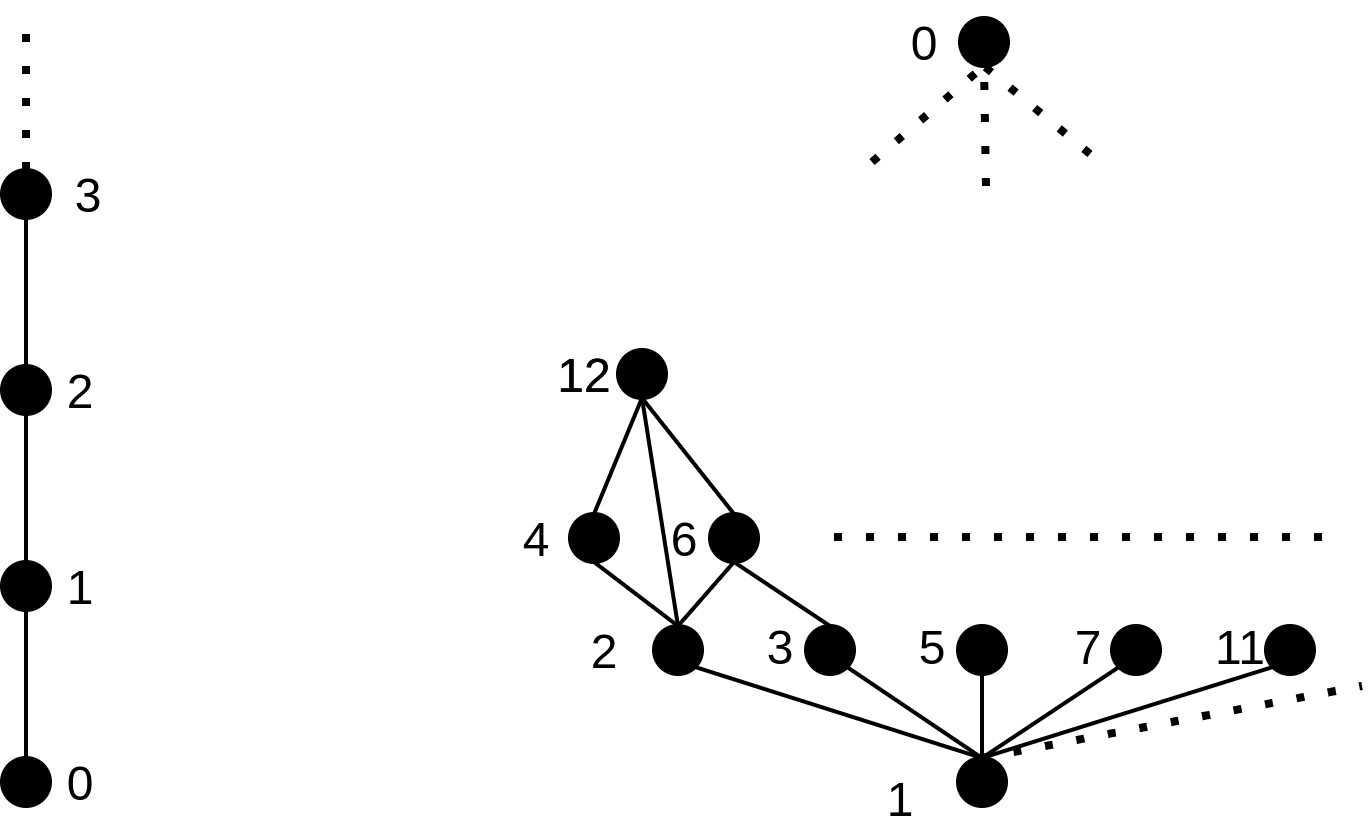
\includegraphics[width=0.5\textwidth]{images/reticolo2.png}
  \caption{Due relazioni d'ordine.}
  \label{figure:relazionireticoli}
\end{figure}

Nella Figura \ref{figure:relazionireticoli} si può vedere una rappresentazione 
(tramite reticoli, definiti a seguire) delle due relazioni d'ordine. 
La prima, quella totale, è rappresentata a destra: si può notare come sia 
``lineare'' a confronto della seconda, parziale, che è rappresentata a 
sinistra: quest'ultima infatti si dirama: alla base ha $1$, il numero che 
divide tutti gli altri; al primo ``strato'' ha tutti i numeri primi, 
il secondo i multipli dei multipli dei numeri primi (che saranno comunque collegati 
ai numeri primi, in quanto saranno divisibili anche per essi) e, commettendo 
un abuso che solitamente viene concesso, in cima vi è il numero $0$ che è divisibile 
da tutti gli altri, benché non sia divisibile per sé stesso. 

\subsubsection{Reticoli}
Un insieme $P$ con una relazione d'ordine (parziale) $\leq$, 
notato $(P, \leq)$ è detto insieme parzialmente ordinato 
o, in inglese, partially ordered set (\textit{poset}). 
L'insieme delle classi di equivalenza 
delle formule è un insieme parzialmente ordinato con delle peculiarità. 

Tra tutti i \textit{poset}, ci interessano quelli con alcune particolari proprietà 
strutturali, chiamati \textbf{reticoli}. 

\begin{figure}[!h]
  \centering 
  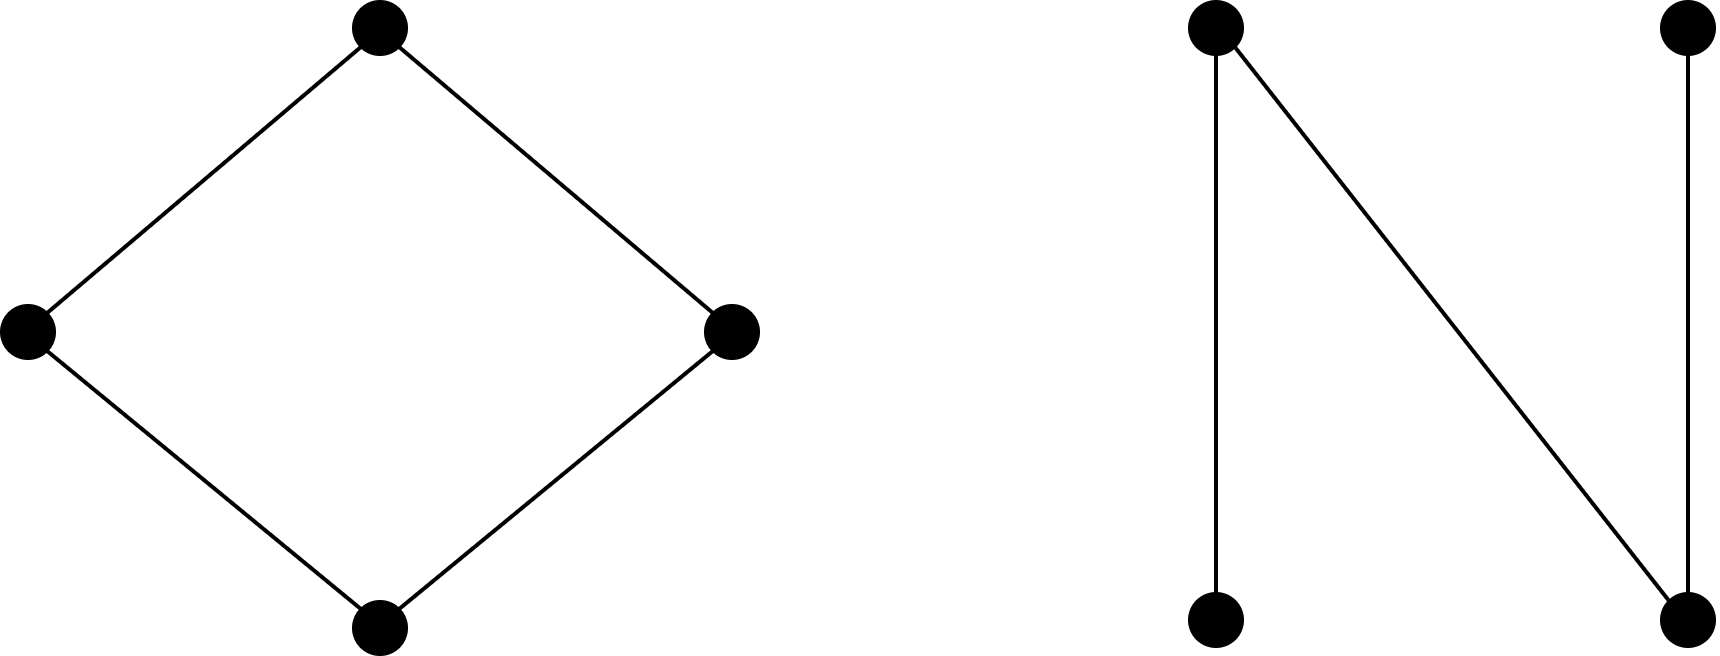
\includegraphics[width=0.5\textwidth]{images/reticolo.png}
  \caption{Due reticoli.}
  \label{figure:reticolo}
\end{figure}


La Figura \ref{figure:reticolo} riporta due immagini. 
Non entrambi sono reticoli: quello più a destra, infatti, non lo è. 
Cosa li distingue? La proprietà strutturale (più importante per i nostri 
scopi) che li divide, è che per quello più a sinistra, il reticolo, data 
ogni qualsiasi coppia di elementi possibile, si può sempre trovare 
quale dei due sia il minimo elemento che è più grande della coppia e il 
massimo elemento che è più piccolo della coppia. Questo non avviene nell'altro 
caso, infatti i due elementi ``in alto'', non hanno un minimo elemento 
più grande di loro, mentre i due elementi ``in basso'' non hanno un massimo 
elemento più piccolo di loro. In altre parole, non hanno 
\textbf{estremi inferiori} ed \textbf{estremi superiori}, che sono 
invece la proprietà fondamentale dei reticoli. 

Si definiscono quindi questi due concetti. 

\begin{defi}[Estremo inferiore]
        Dati due elementi $x, y$ appartenti ad un insieme 
        parzialmente ordinato $(P, \leq)$, si definisce 
        $$
        \inf(\{x,y\}) = \max\{z \in (P, \leq): z \leq x \text{ e } z \leq y\}
        $$
\end{defi}
e si definisce, analogamente 
\begin{defi}[Estremo superiore]
        Dati due elementi $x, y$ appartenti ad un insieme 
        parzialmente ordinato $(P, \leq)$, si definisce 
        $$
        \sup(\{x,y\}) = \min\{z \in (P, \leq): x \leq z \text{ e } y \leq z\}
        $$
\end{defi}
Si possono generalizzare $\inf$ e $\sup$ ad un insieme $S \subseteq P$, con 
$P$ poset $(P, \leq)$, affermando che 
$$
        \inf(S) = \max\{z \in (P, \leq): z \leq s \forall s \in S\}
$$
e 
$$
        \sup(S) = \min\{z \in (P, \leq): s \leq z \forall s \in S\}
$$
A questo punto si può definire il massimo di un insieme (e analogamente il minimo) 
definendolo come 
$$
        \max(S) = \sup(S) \text{ se } \sup(S) \in S
$$
Si può ora definire formalmente un reticolo: 
\begin{defi}[Reticolo]
Un reticolo è un insieme parzialmente ordinato $(R, \leq)$ tale che 
per ogni $x, y \in R$ esistono $\inf(\{x,y\})$ e $\sup(\{x,y\})$. 
\end{defi}

\noindent 
Dopo aver definito i reticoli, si definisce un'ulteriore struttura, necessaria 
per concludere l'argomento dell'Algebrizzazione della Logica Booleana. 

\subsection{Struttura Algebrica}

Dato un insieme $S$ e
date le operazioni $*_1, *_2, \cdots, *_n$ delle operazioni 
in $S$, allora $(S, *_1, *_2, \cdots, *_n)$ è una \textbf{struttura algebrica}. 

Visto come una struttura algebrica, un reticolo 
è $(R, \sqcup, \sqcap)$, con $\sqcup, \sqcap$ operazioni 
$\sqcup: R^2 \rightarrow R$ e $ \sqcap: R^2 \rightarrow R$, tale che 
le due operazioni siano commutative, associative e 
valga l'assorbento. 
Ogni reticolo visto come insieme parzialmente 
ordinato è anche una struttura algebrica 
$$
(R, \leq) \iff (R, \sqcup, \sqcap)
$$
Infatti si può associare una struttura algebrica 
a una struttura ordinata 
(ossia si può definire il reticolo come 
struttura algebrica partendo dalla sua definizione come 
poset) definendo $R\equiv R$, 
$a \sqcup b := \inf \{a,b\}$ e $a \sqcap b := \sup \{a,b\}$ 
per ogni $a,b \in R$. Si verifichino 
le proprietà di 
commutatività, assorbimento e associatività. 

Si può associare una struttura ordinata 
a ogni struttura algebrica (ossia si può definire 
il reticolo come poset partendo dalla 
sua definizione come struttura algebrica)
definendo $R \equiv R$ e 
sostanzialmente definendo quando accade che $a \leq b$.

Per ogni $a, b \in R$ si definisce un operatore 
$ a = a \sqcap b $ o equivalentemente $b = a \sqcup b$. 
Si deve verificare che $a \leq b \iff a = a \sqcap b$ sia tale 
che $\leq$ sia riflessiva, antisimmetrica e transitiva, 
dalla quale deriva che $R$ è un poset. 
Per concludere che $R$ sia in particolare un poset-reticolo bisogna mostrare 
che per ogni coppia $a,b \in R$ esiste $\inf$ e $\sup$. 
Sia allora $c \leq a$ e $ c \leq b$: bisogna mostrare 
che $c \leq \inf\{a,b\}$, in genere 
$c \leq a \sqcap b$. 
Ma $c = a \sqcap c = a \sqcap (b \sqcap c)$ per la definizione di 
$\leq$; si può allora scrivere 
$$
\text{ per associatività }(a \sqcap b) \sqcap c \iff c \leq a \sqcap b 
$$
per definizione di $\leq$. Per il $\sup$ si ragiona 
in modo analogo. 


\subsection{Definizione di Algebra Booleana}
A questo punto, siamo finalmente pronti per definire cosa sia l'Algebra Booleana.
\begin{defi}{Algebra Booleana}
L'Algebra Booleana è un sistema $(S, \sqcap, \sqcup, 0, 1, ()^c)$ operazioni 
tali che $(S,\sqcup,\sqcap)$ sia un reticolo limitato, complementato, 
distributivo:
\begin{itemize}
        \item \textbf{limitato} in quanto per ogni $a \in S$ si ha $a \sqcap 0 = a$ e $a \sqcap 1 = a$ ($ a \geq 0$ e $ a \leq 1$); 
        \item \textbf{distributivo} in quanto per ogni $a,b c \in S$ si ha 
                $$
                a \sqcap (b \sqcup c) = (a \sqcap b) \sqcup (a \sqcap c)
                $$ e 
                $$
                a \sqcup (b \sqcap c) = (a \sqcup b) \sqcap ( a \sqcup c)
                $$
        \item \textbf{complementato} in quanto $a \sqcap a^c = 0$ e $a \sqcup a^c = 1$. 
\end{itemize}
\end{defi}

Un esempio è il seguente: dato un insieme $A$ si consideri 
$(P(A), \cup, \cap, \emptyset, A, ()^c)$ e si ha 
$(P(A), \subseteq)$ tale che $A \subseteq B \iff A = A \cap B$. 

\paragraph{Esercizio} 
Sia $A$ un insieme infinito e sia $F(A)$
l'insieme dei suoi sottoinsiemi finiti o complementi di insiemi 
finiti. Si dimostri che $(F(A), \cup, \cap, \emptyset, A, ()^c)$ è un algebra booleana. 
Un altro esempio di algebra 
booleana è quella dei valori di verità $(\{0,1\}, \min, \max, 0, 2, 1-\_)$. 

\subsubsection{Algebra di Lindenbaum}
L'algebra delle formule, chiama anche \textbf{Algebra di 
Lindenbaum delle Formule}, è definito $(F_L/\equiv, \land, \lor, \bot, \top, \neg)$. 
Dato che $\equiv$ è una congruenza, si può quindi procedere a definire
$$
A,B \in F_L [A]_{\equiv} \land [B]_{\equiv} = [A \land B]_{\equiv}
$$
$$
A,B \in F_L [A]_{\equiv} \lor [B]_{\equiv} = [A \lor B]_{\equiv}
$$
$$
A,B \in F_L [A]_{\equiv} \rightarrow [B]_{\equiv} = [A \rightarrow B]_{\equiv}
$$
$$
A \in F_L \neg [A]_{\equiv} = [\neg A]_{\equiv}
$$
$$
[\top]_{\equiv} = \text{ tautologie}
$$
$$
[\bot]_{\equiv} = \text{ contraddizioni}
$$
La cardinalità dell'insieme delle classi di equivalenza scrivibili con $n$
variabili è 

$$
|F^{(n)}/\equiv| = 2 ^ {2^n} = |\{F: \{0,1\}^n \rightarrow \{0,1\}\}|
$$

\subsection{Funzioni Termine}
Al fine di arrivare ad un discorso completo sulle Forme Normali, 
si continua a ragionare sulle classi d'equivalenza delle formule e la 
loro struttura, ora da un punto di vista che sembra essere diverso 
ma che in conclusione si riunirà con quanto detto precedentemente. 

Si rifletta sul significato di 
$$
\models F \iff \forall \mathfrak{v}: L \rightarrow \{0,1\} ~~~  \mathfrak{v}(F) = 1
$$
in termini ``computazionali'' significa \textit{tenere fermo} l'argomento 
($F$) e far cambiare le funzioni. Sarebbe comodo scambiare i ruoli, nel 
senso che si vorrebbe che la formula diventasse una funzione, in qualche modo,
e gli assegnamenti degli argomenti. 
Sia ora $A \in F_L$ una formula. Si chiama $Var(A) \subseteq L$ l'insieme delle lettere 
proposizionali che occorrono in $A$ tale che 
$Var(A) \subseteq \{p_1, p_2, \cdots, p_n\}$ per un qualche naturale $n$.  
Sia ora $\hat{A}$ una funzione definita come 
$$
\hat{A} : \{0,1\}^n \rightarrow \{0,1\}
$$
tale che 
$$
\forall \mathfrak{v}:L \rightarrow \{0,1\} ~~~~ \hat{A}(\mathfrak{v}(p_1), \mathfrak{v}(p_2), \cdots, \mathfrak{v}(p_n)) = \tilde{\mathfrak{v}}(A)
$$
la fuzione $\hat{A}$ si chiama \textbf{funzione termine} e, per definirla formalmente, 
si procede per induzione. 
\paragraph{Caso base:} 
Sia 
$ A = p_i$, con $p_i \in \{p_1, p_2, \cdots, p_n\}$ un letterale.
Allora 
$$
\hat{A} := \hat{p_i} : \{0,1\}^n \rightarrow \{0,1\}
$$ 
dove, per ogni $(t_1, \cdots, t_n)$ si ha 
$$
\hat{p_i}(t_1, \cdots, t_n) = t_i
$$
ossia l'$i$-esima proiezione. 
Quindi, nel caso base, $\forall \mathfrak{v}: L \rightarrow \{0,1\}$ si ha che 
$$
\hat{A} = \hat{p_i}(\mathfrak{v}(p_1), \cdots, \mathfrak{v}(p_n)) = \mathfrak{v}(p_i)
$$
\paragraph{Passo induttivo:}
\begin{itemize}
        \item Se $A = \neg B$ allora $\hat{A}(t_1, \cdots, t_n) =  1 - \hat{B}(t_1, \cdots, t_n)$. 

        \item Se $A = B \land C$ allora $\hat{A}(t_1, \cdots, t_n) = min \{\hat{B}(t_1, \cdots, t_n), \hat{C}(t_1, \cdots, t_n)\}$. 
        \item Se $A = B \lor C$ allora $\hat{A}(t_1, \cdots, t_n) = max \{\hat{B}(t_1, \cdots, t_n), \hat{C}(t_1, \cdots, t_n)\}$. 
        \item Se $A = B \rightarrow C$ allora $\hat{A}(t_1, \cdots, t_n) = max \{1 - \hat{B}(t_1, \cdots, t_n), \hat{C}(t_1, \cdots, t_n)\}$. 
\end{itemize}

Ora si può trasformare la riflessione iniziale in termini di Funzioni Termine: 
$$
\models F \iff \hat{F}(t_1, \cdots, t_n) = 1 \forall (t_1, \cdots, t_n)
$$
e l'equivalenza logica: 
$$
[F]_{\equiv} = [G]_{\equiv} \iff F \equiv G \iff \hat{F}(t_1, \cdots, t_n) = \hat{G}(t_1, \cdots, t_n) \forall t_i
$$
A questo punto, potrebbo avere una definizione diversa di Algebra Booleana da 
esporre, che in realtà è la stessa Algebra di Lindenbaum scritta in maniera 
diversa
\begin{defi}[Algebra Booleana su Funzioni Termine]
$$
\hat{F}_L = (\{\hat{A}: \{0,1\}^n \rightarrow \{0,1\}, A \in F_L\}, \land, \lor, \neg, \bot, \top) 
$$
dove i significati degli operatori sono quelli espressi precedentemente. 
\end{defi}

Eccetto la natura ``fisica'', l'Algebra di Lindenbaum e l'Algebra Booleana su 
Funzioni Termine sui
primi $n$ termini sono \textbf{isomorfe}. 

\subsection{Teorema di Completezza Funzionale}
Concentriamoci sull'Algebra appena espressa
$$
\hat{F}_L = (\{\hat{A}: \{0,1\}^n \rightarrow \{0,1\}, A \in F_L\}, \land, \lor, \neg, \bot, \top) 
$$
e costruiamo un'altra Algebra definita come
$$
Funz^{(n)} = (\{F: \{0,1\}^{(n)} \rightarrow \{0,1\}\}, \land, \lor, \neg, \bot, \top)
$$
Che rapporto sussiste tra le due Algebre?
La prima ha come universo l'insieme di tutte le Funzioni Termine per ogni 
formula $A \in F_L$, mentre la seconda ha come universo tutte le funzioni
$$
F: \{0,1\}^n \rightarrow \{0,1\}
$$
per ogni $n \in \mathbb{N}$.
Sicuramente, data la restrizione, si può affermare che 
$$
\hat{F}_L^{(n)} \subseteq Funz^{(n)}
$$
Si dimostra, ora, che vale anche
$$
\hat{F}_L^{(n)} \supseteq Funz^{(n)}
$$
Questo fatto prende il nome di \textbf{Teorema di Completezza Funzionale}. 
A parole, ciò che si afferma è che ogni funzione 
$$
F: \{0,1\}^n \rightarrow \{0,1\}
$$
è esprimibile come una formula $F \in F_L$.
Chiaramente, dimostrando questo, si ha che le due Algebre esposte 
sono in realtà la stessa, ossia sono \textbf{isomorfe}. 
\begin{teo}[di Completezza Funzionale]
        Per ogni $n \in \mathbb{N}$
        $$
                \hat{F}_L^{(n)} \supseteq Funz^{(n)}
        $$
\end{teo}

La dimostrazione consiste nel fornire un metodo per ottenere una Funzione Termine 
$$
\hat{F} = F
$$
per ogni formula $F: \{0,1\}^{n} \rightarrow \{0,1\}$. 
\begin{proof}
        Sia data una formula 
        $$
        F: \{0,1\}^{n} \rightarrow \{0,1\}
        $$
        La cardinalità del dominio di $F$ è 
        $$
        |Dom(F)| =  2^{n}
        $$
        e per ogni combinazione degli $n$ argomenti esiste un certo risultato 
        associato, che definiamo $b_i ~~ i=0,\cdots,2^{n}-1$. 
        Costruiamo una formula $F \in F_L$ in modo tale che $ \hat{F} = F$. 
        Se $F(t_1, \cdots, t_n) = 0$ per ogni $(t_1, \cdots, t_n)$, allora 
        si può semplicemente scegliere $F = \bot$, analogamente nel caso 
        in cui sia sempre vera. 
        
        Altrimenti, sia 
        $$
        I \subseteq \{0, 1, \cdots, 2^{n}-1\}
        $$
        tale che 
        $$
        i \in I \iff b_i = 1
        $$
        (intuitivamente, $I$ contiene i numeri delle ``righe'' della tabella 
        di verità della funzione $F$ in cui l'immagine è il numero $1$).
        Per ogni $i \in I$ si considera la $i$-esimo elemento del 
        dominio di $F$, che è composto come 
        $$
        (a_{i1}, a_{i2}, \cdots, a_{in})
        $$
        e per ogni $j \in \{1, \cdots, n\}$ si definisce
        $$
        A_{ij} = 
        \begin{cases}
                p_j & a_{ij} = 1 \\
                \neg p_j & a_{ij} = 0
        \end{cases}
        $$
        Si noti che $A_{ij} \in F_L$. Si pone, ora
        $$
        F = \lor_{i\in I}\land_{j} A_{ij}
        $$
        E si può mostrare $\hat{F} = F$: chiaramente, 
        $$
        \land_{j = 1}^{n} \hat{A}_{ij}(t_1, \cdots, t_n) = 1 
        $$
        se e solo se 
        $$
        (t_1, \cdots, t_n) = (a_{i1}, \cdots, a_{in})
        $$
        Altrettanto ovviamente, considerando 
        $$
        (A_{i1} \land A_{i2} \land \cdots \land A_{in})
        $$
        nel ``punto'' $(a_{i1}, a_{i2}, \cdots, a_{in})$ 
        si sa che il suo valore di verità è $1$, ed è l'unico caso in cui 
        sia così; in definitiva, 
        $$
        \hat{F} = \lor_{i\in I}\land_{j} A_{ij}(t_1, \cdots, t_n) = 1 \iff  i \in I
        $$
        e $\hat{F} = F$.
\end{proof}

\subsubsection{Considerazioni sul Teorema di Completezza Funzionale}
Per come è stato provato il Teorema di Completezza Funzionale, la funzione può 
essere espressa 
$$
F = \lor_{i \in I} \land_{j = 1}^{n} A_{ij}
$$
e 
$$
G = \land_{i \in J} \lor_{j = 1}^{n} B_{ij}
$$
definendo 
$$
J \subseteq {0, \cdots, 2^n -1 } ~~j \in J \iff b_j = 0
$$
e 
$$
B_{ij} =
\begin{cases}
        \neg p_j & a_{ij} = 1 \\
        p_j & a_{ij} = 0 \\

\end{cases}
$$
Si ha che $\hat{F} = F = \hat{G}$\footnote{Ciò che è stato 
        fatto è esattamente uguale alla costruzione dei minterm 
e maxterm per una data tavola di verità.}, è pertanto una dimostrazione dell'esistenza 
delle \textbf{forme normali} e si può concludere che il Teorema di Completezza 
Formale sia un Teorema di Forma Normale. 

Sebbene il Teorema possa sembrare banale, in quanto la sua dimostrazione è
semplice, il suo contenuto non è nullo né scontato. Un esempio di mancanza 
funzionale è già presente nella Logica Proposizionale stessa, nonostante 
la dimostrazione precedente, rimuovendo il vincolo su $n$ e definendo
$$
Funz^{\omega} := \{f:\{0,1\}^{\omega} \rightarrow \{0,1\}\}
$$
con $\omega = |\mathbb{N}|$, in altre parole l'insieme di tutte le successioni 
infinite di valori $\{0,1\}$. Se valesse il Teorema di Completezza Funzionale 
anche in questo caso, si dovrebbe poter affermare che tale insieme 
è incluso nelle classi di equivalenza scritte nelle classi di equivalenza 
delle formule scritte con $\omega$ variabili: 
$$
Funz^{\omega} \subseteq \hat{F}^{\omega}_{L} = F_L^{\omega}/\equiv
$$
Ma in realtà
$$
|Funz^{\omega}| = |\mathbb{R}| \geq |\mathbb{N}| = |F_L^{\omega}/\equiv|
$$
e pertanto non è valido. 

\paragraph{Forme Normali Canoniche}
Le forme normali che abbiamo trovato non sono desiderabili per gli scopi 
futuri, in quanto sono molto prolisse: ognuno degli $A_{ij}$ menziona 
tutte le lettere proposizionali $p_1, \cdots, p_n$ (analogamente per le 
forme congiuntive) ed è infatti chiamata Forma Normale Disgiuntiva (or di and) 
\textbf{Canonica} o \textbf{Completa}. Per esempio, siano date tre variabili 
$p_1$, $p_2$ e $p_3$, si vuole costruire la formula 
$$
F(t_1, t_2, t_3) = t_1
$$
è chiaro che la formula più ``corta'' è $\hat{F} = t_1$, ma con la forma 
canonica il risultato è 
$$
\hat{F} = (p_1 \land \neg p_2 \land \neg p_3) \lor (p_1 \land \neg p_2 \land p_3) \lor (p_1 \land p_2 \land \neg p_3) \lor (p_1 \land p_2 \land p_3)
$$
molto più lunga.

\paragraph{Insieme funzionalmente completo di connettivi}
C'è un'altra nozione, legata alla Completezza Funzionale, che è molto interessante, 
ossia la nozione di \textbf{insieme funzionalmente completo di connettivi}. 
\begin{defi}[Insieme funzionalmente completo di connettivi]
        Un insieme 
        $$
        C \subseteq \{\land, \lor, \rightarrow, \neg, \iff, \bot, \top\}
        $$
è definito funzionalmente complete se per ogni $F \in F_L$ esiste una $G \in F_L$ 
scritto usando solo i connettivi in $C$ tale che $F \equiv G$ e $\hat{F} = \hat{G}$, 
ossia $[F]_{\equiv} = [G]_{\equiv}$. 
\end{defi}

Un insieme di connettivi funzionalmente 
completo è dato dal Teorema di Completezza Funzionale stesso, ossia 
$C = \{\land, \lor, \neg\}$, che è funzionalmente completo grazie 
al Teorema di Completezza Funzionale. Si può mostrare facilmente che 
anche $\{\neg, \land\}$ e $\{\neg, \lor\}$ sono completi (in quanto, grazie alle 
leggi di De Morgan, $(A \lor B) = \neg (\neg A \land \neg B)$). Questi non 
sono gli unici insiemi funzionalmente completi: 
$\{\neg, \rightarrow\}$ (in quanto $(A \land B) \equiv \neg (A \rightarrow \neg B)$ 
e $(A \lor B) \equiv ((\neg A) \rightarrow B)$ 
e $\{\rightarrow, \bot\}$. In particolare, un insieme composto da un 
solo connettivo, il \texttt{nand}, è anch'esso funzionalmente completo, 
in quanto ogni altro connettivo è ricostruibile utilizzando solo 
$$
A \barwedge B = \neg (A \land B)
$$
infatti $\neg A \equiv A \barwedge A$ e, ovviamente, $A \land B \equiv \neg ( A \barwedge B)$ 
per definizione. 

\section{Forme Normali}
Dopo averle introdotte col Teorema di Completezza Funzionale, possiamo 
passare ad un esame più approfondito delle Forme Normali.
Le Forme Normali Congiuntive e Disgiuntive Canoniche sono 
esageratamente prolisse. Sarebbe utile conservare l'idea delle Forme Normali 
con formule più succinte. 

\subsection{Forma Normale Negata}
Una terza forma normale, chiamata \textbf{Negation 
Normal Form} (NNF) che, per definizione, è l'insieme delle formule 
che rispettano le seguenti proprietà: 
\begin{itemize}
  \item non contiene $\rightarrow$ 
  \item $\neg$ occorre solo applicato a lettere proposizionali
\end{itemize}
quindi, per esempio 
$$ 
p_1 \land \neg(p_2 \lor p_3)
$$
non è una NNF, mentre 
$$
p_1 \land (\neg p_2 \lor \neg p_3)
$$
è una NNF. 
\begin{lem}
Ogni formula $F \in F_L$ è equivalente a una $F^{N} \in NNF$. 
\end{lem}
\begin{proof}
Per provare il lemma, descriviamo come trasformare $F$ in $F^{N}$ in un numero 
finito di passi, dove ogni passo produce una formula equivalente alla precedente. 
Per ottenere la sequenza si applica ad ogni passo una delle seguenti 
trasformazioni: 

\begin{enumerate}
  \item $C \rightarrow D$ in $(\neg C) \land D$
  \item $\neg \neg C$ in $C$
  \item $\neg(C \lor D)$ in $\neg C \land \neg D$
  \item $\neg (C \land D)$ in $\neg C \lor \neg D$
\end{enumerate}

Un'osservazione preliminare su questo algoritmo è che si può mostrare che applicando 
le quattro regole in un ordine qualsiasi si ottiene sempre $F^{N} \in NNF$. 
Si mostrerà che partendo da $(1)$ e applicando le altre trasformazioni si possa 
arrivare a $F^{N}$: sia data $F \in F_L$. In un numero finito di applicazioni 
di $(1)$ si ottiene una $F'$ in IFNF (Implication-Free Normal Form), equivalente 
a $F$. 

Si introduce una misura di \textit{distanza}: si definisce 
$i(E)$ come il numero di connettivi $\rightarrow$ nella formula $E$. 
Si ha, quindi, 
che $E \in IFNF \iff i(E) = 0$. Inoltre, se $E \notin IFNF$, allora 
$E'$ ottenuta applicando $(1)$ su $E$ deve avere $i(E) > i(E')$. 
\`E chiaro che $F \equiv F'$ poiché l'applicazione di $(1)$ è semplicemente 
l'applicazione di una equivalenza eseguita grazie al Teorema di Sostituzione. 
Quindi, in un certo numero di passi  si ha
$$ 
F = F_0 \equiv \cdots \equiv F' (\in IFNF) \equiv F_i \equiv \cdots \equiv F_n (\in NNF)
$$
e si nota che le applicazioni di $(2)$, $(3)$ e $(4)$ trattano tutte equivalenze logiche. Ciò 
che bisogna dimostrare è che la sequenza di trasformazioni termini, ossia l'algoritmo 
non è infinito ($n \in \mathbb{N}$). 
Per dimostrare che l'algoritmo termina, sia ora $A \in F_L$ 
e si definisce 
$$ 
l(A) = \text{ numero di occorrenze di connettivi in } A
$$ 
e 
$$
m(E) = \sum_{\neg A \in E} l(A)
$$
dove la notazione $\neg A \in E$ indica che $\neg A$ sia una sottoformula.
Si noti che 
$$
m(E) = 0 \iff E \in NNF
$$
in quanto 
$$
\begin{cases}
        E \in NNF  & \neg A \in E \iff A \in L \iff l(A) = 0 \iff m(E) = 0\\
                m(E) = 0 & \sum_{\neg A \in E} l(A) = 0 \iff l(A) = 0 \iff A \in L 
\end{cases}
$$
In un passaggio eseguito con una delle $(2), (3), (4)$ generando 
$$
E \leadsto E'
$$
si ha che $m(E) > m(E')$. Se si riesce a dimostrare quest'ultima affermazione, 
allora si dimostra automaticamente che il procedimento termina in un numero 
finito di passi. 
\paragraph{(2)} 
$$
\neg \neg C \leadsto C
$$
In questo caso 

\begin{align*}
        m(\neg \neg C) = \sum_{\neg A \in \neg \neg C} l(A) &= l(\neg C) + \sum_{\neg A \in \neg C} l(A) \\
                                                            & =l(C) + 1 + l(C) + \sum_{\neg A \in C} l(A)
\end{align*}
mentre 
\begin{align*}
        m(C) = \sum_{\neg A \in C} l(A) < 1 + 2*l(c) + \sum_{\neg A \in C} l(A)
\end{align*}

\paragraph{(3)}
$$
\neg (C \land D) \leadsto \neg C \land D
$$
In questo caso 
\begin{align*}
        m(\neg (C \land D)) = 1 + \sum_{\neg A \in (C \land D)} = l(C) + l(D) + 1 + \sum_{\neg A \in C} l(A) + \sum_{\neg A \in D} l(A)
\end{align*}
mentre 
\begin{align*}
        m(\neg C\lor \neg D) = l(C) + l(D) + \sum_{\neg A \in C} l(A) + \sum_{\neg A \in D} l(A) < 1 + \sum_{\neg A \in C} l(A) + \sum_{\neg A \in D} l(A) 
\end{align*}
Analogamente per $(4)$. Data una formula $F \in F_L$, si può costruire una successione 
finita 
$$ 
F = F_0 \equiv \cdots \equiv F' (\in IFNF) \equiv F_i \equiv \cdots \equiv F_n (\in NNF)
$$
e ovviamente $F \equiv F_n$, per un qualche $n \in \mathbb{N}$. 
\end{proof}

\subsection{Forma Normale Congiuntiva e Disgiuntiva}
Le FNC, Forme Normali Congiuntive o CNF, sono un superset delle CNF complete o canoniche.
\begin{defi}[Letterale]
Un \textbf{letterale} è una formula nella forma $p$ o $\neg p$ per qualche 
lettera proposizionale $p$ - o è una lettera proposizionale o è la sua negata. 
La definizione di \textbf{letterale opposto} a uno dato è, dato $A$ letterale, 
l'opposto di $A$
$$
\bar{A} = 
\begin{cases}
  \neg p & A = p \\
  p & A = \neg p
\end{cases}
$$
\end{defi}
\begin{defi}[Clausola]
Una \textbf{clausola} è una disgiunzione di un numero finito di letterali come 
$$
l_1 \lor l_2 \cdots \lor l_k
$$
dove ogni $l_i$ è un letterale. 
\end{defi}
\begin{defi}[FNC]
Una \textbf{forma normale congiuntiva} è una congiunzione di un numero finito di 
clausole, come 
$$
c_1 \land c_2 \land \cdots \land c_h
$$
dove ogni $c_j$ è una clausola. 
\end{defi}
\begin{defi}[Clausola vuota]
Una \textbf{clausola vuota} $\qedsymbol$ è definita come la disgiunzione 
di zero letterali. 
\end{defi}

Questo concetto è importante e non va confuso col concetto 
di \textbf{CNF vuota} $\emptyset$, definita come la congiunzione di zero clausole. 
Prendendo una sequenza di letterali e formule
\begin{align*}
\qedsymbol \\
l_1 \\
l_1 \lor l_2 \\
l_1 \lor l_2 \lor l_3 \\
l_1 \lor l_2 \lor l_3 \lor l_4
\end{align*}
possiamo affermare che la catena di implicazioni dall'alto verso il basso 
è una catena di tautologie, infatti
ogni assegnamento che soddisfa una formula soddisfa anche la successiva, verso 
il basso - seguendo questa definizione la clausola vuota è insoddisfacibile e 
pertanto, per noi, è $\qedsymbol \equiv \bot$.

Per l'insieme di CNF vuote, si ha 
\begin{align*}
\emptyset \\
c_1 \\
c_1 \land c_2 \\
c_1 \land c_2 \land c_3\\
c_1 \land c_2 \land c_3 \land c_4
\end{align*}
qui, al contrario, ogni assegnamento che soddisfa una clausola soddisfa anche la 
precedente, verso l'alto - seguendo questa definizione la CNF vuota è per 
definizione soddisfacibile ed è, in realtà, soddisfatta da ogni assegnamento 
e $\emptyset \equiv \top$. 

\begin{defi}[Forma Normale Disgiuntiva]
Le FND, Forme Normali Disgiuntive o DNF sono definite come disgiunzione di 
un numero finito di formule 
$$
D_1 \lor D_2 \lor \cdots \lor D_n
$$
dove ogni $D_i$ è una congiunzione chiamata \textbf{co-clausola} di un numero finito 
$$
l_1 \land l_2 \land \cdots \land l_v
$$
di letterali. 
\end{defi}

si tratta, quindi, di una struttura duale rispetto alle CNF. 
Si noti la terminologia speciale per le CNF: questa terminologia è riservata 
alle CNF in quanto la dualità tra CNF e DNG verrà spezzata. 

\begin{lem}
Ogni formula $F \in F_L$ è logicamente equivalente a una formula $F^c \in CNF$ 
e a una formula $F^d \in DNF$.
\end{lem}

Questo è già stato dimostrato grazie al teorema 
di completezza funzionale, che tuttavia utilizzava le CNF e DNF complete: una 
versione alternativa della dimostrazione è la seguente, per induzione strutturale 
su $F$. 
\subsubsection{Dimostrazione esistenza DNF/CNF}
\begin{itemize}
        \item \textbf{base induttiva:} se $F = p, p \in L$ allora $p = p^c = p^d$. 
        \item \textbf{passo induttivo:} 
                \begin{enumerate}
                        \item se $F = \neg G$ per ipotesi induttiva si ha $G^c \equiv G$, $G^d \equiv G$. 
                                Allora, se 
                        \[
                                G = C_1 \land C_2 \land \cdots \land C_n
                        \]
                                con 
                                $$
                                C_i = l_{i1} \lor \cdots \lor l_{ik_i}
                                $$
                                si ha che 
                                \begin{align*}
                                        \neg G^c &\equiv \neg (C_1 \land \cdots \land C_n) \\
                                        \text{(DeMorgan) } &\equiv \neg C_1 \lor \neg C_2 \lor \cdots \lor \neg C_n \\
                                        \text{(DeMorgan) } &\rightarrow \neg C_i \equiv \neg l_{i1} \land \cdots \land \neg l_{ik_i} \\
                                                           & \rightarrow \neg G^c \in DNF 
                                \end{align*}
                                e similmente
                                \begin{align*}
                                        \neg G^d &\equiv \neg (C_1 \lor \cdots \lor C_n) \\
                                        \text{(DeMorgan) } &\equiv \neg C_1 \land \neg C_2 \land \cdots \land \neg C_n \\
                                        \text{(DeMorgan) } &\rightarrow \neg C_i \equiv \neg l_{i1} \lor \cdots \lor \neg l_{ik_i} \\
                                                           & \rightarrow \neg G^d \in CNF
                                \end{align*}
                                Quindi, ``scambiandosi'', esistono sia $(\neg G)^c \equiv (\neg G^d)$ 
                                e $(\neg G)^d \equiv (\neg G^c)$. 
                        \item se $F = (G \land H)$, per ipotesi induttiva si hanno
                                $G^c \equiv G$, $G^d \equiv G$, $H^c \equiv H$ e 
                                $H^d \equiv H$. 
                                Si definisce, allora 
                                \begin{align*}
                                        F &\equiv F^c  \equiv G^c \land H^c
                                \end{align*}
                                banalmente, mentre 
                                \begin{align*}
                                        F &\equiv F^d \\
                                          &\equiv (G_1 \lor \cdots \lor C_n) \land (H_1 \lor \cdots \lor H_k) \\
                                        \text{(Dist. gen.)} &\equiv \lor_{i,j}(G_i \land H_j) \\
                                                            &\rightarrow \lor_{i=1}^n \lor_{j=1}^k (G_i \land H_i) \in DNF
                                \end{align*}
                        \item se $F = (G \lor H)$, per ipotesi induttiva si hanno
                                $G^c \equiv G$, $G^d \equiv G$, $H^c \equiv H$ e 
                                $H^d \equiv H$.                 
                                Si può definire, allora 
                                \begin{align*}
                                        F &\equiv F^d  \equiv G^d \land H^d
                                \end{align*}
                                banalmente, mentre 
                                \begin{align*}
                                        F &\equiv F^c \\
                                          &\equiv (G_1 \land \cdots \land C_n) \lor (H_1 \land \cdots \land H_k) \\
                                        \text{(Dist. gen.)} &\equiv \land_{i,j}(G_i \lor H_j) \\
                                                            &\rightarrow \land_{i=1}^n \land_{j=1}^k (G_i \lor H_i) \in CNF
                                \end{align*}                
                \end{enumerate}
\end{itemize}

Si nota, tuttavia, che muoversi tra DNF e CNF causa un notevole allungamento 
delle formule: per esempio, avendo 
\begin{align*}
        \lor_{i = 1}^{n} (p_i \land q_i) \equiv \land_{i = 1}^{2^n}(l_{i1} \lor \cdots \lor l_{in})
\end{align*}
quindi c'è una dilatazione esponenziale. Questo è ovviamente un bel problema. 
Ci sono algoritmi più intelligenti per generare formule DNF o CNF più corte? 
Purtroppo no. 
